\documentclass{article}
\usepackage{tikz}
\usepackage{pgfplots}
\pgfplotsset{compat=1.18}
\begin{document}
\section*{TikZ and pgfplots}

\emph{In this preview:} TikZ's paths are drawn (lines, curves, circles and arcs, grids, arrows, styles, transforms,
\texttt{\textbackslash foreach}). Text in a picture (nodes) and pgfplots are not drawn yet: such a picture shows as a
placeholder naming what it needs. A full LaTeX run draws them all.

\begin{center}
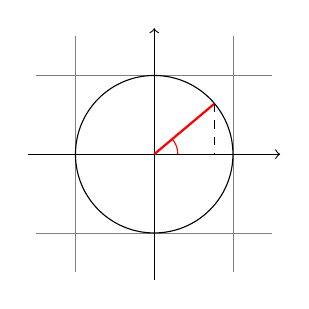
\begin{tikzpicture}
  \draw[help lines] (-1.5,-1.5) grid (1.5,1.5);
  \draw[->] (-1.6,0) -- (1.6,0);
  \draw[->] (0,-1.6) -- (0,1.6);
  \draw (0,0) circle (1);
  \draw[red, thick] (0,0) -- (40:1);
  \draw[red] (0.3,0) arc (0:40:0.3);
  \draw[dashed] (40:1) -- ({cos(40)},0);
\end{tikzpicture}
\end{center}

\begin{center}
\begin{tikzpicture}
  \begin{axis}[xlabel={$x$}, ylabel={$y$}, domain=-2:2, samples=50, legend pos=north west]
    \addplot[blue, thick] {x^2};
    \addlegendentry{$x^2$}
    \addplot[red, dashed] {x^3};
    \addlegendentry{$x^3$}
  \end{axis}
\end{tikzpicture}
\end{center}

\begin{center}
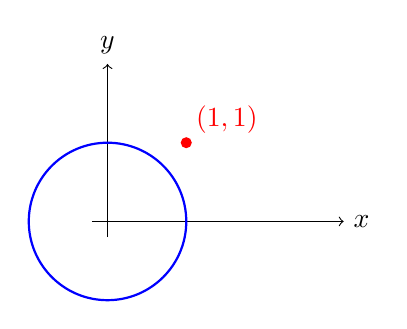
\begin{tikzpicture}
  \draw[->] (-0.2,0) -- (3,0) node[right] {$x$};
  \draw[->] (0,-0.2) -- (0,2) node[above] {$y$};
  \draw[thick, blue] (0,0) circle (1cm);
  \fill[red] (1,1) circle (2pt) node[above right] {$(1,1)$};
\end{tikzpicture}
\end{center}
\end{document}
